% !TEX root = ./HTNotes-Demo.tex
% !TEX program = xelatex
\begin{flushright}
文/似雪飞扬 Lancy
\end{flushright}

\section{引言}
  \begin{quote}
    若人们不相信数学简单,只因他们未意识到生命之复杂。
    \begin{flushright}
      ——约翰·冯·诺依曼
    \end{flushright}
  \end{quote}

  \hspace*{2em}不少大学新生(包括笔者当初)在初次接触高等数学课程时常常感到难以接受,对课程里的数学概念和学习方法感到困惑。本文旨在指出一些观念上的错误,并同读者探讨本科(低年级阶段的)数学课程究竟应当如何学习。

\section{高等数学是什么以及怎么学}

  \hspace*{2em}让我们从高等数学说起。注意,本文的“高等数学”特指微积分。

  \begin{marker}
  {\heiti 第一个问题:“高等数学”是什么,它同我们在高中时期学习的数学有什么联系吗?}
  \end{marker}

  \hspace*{2em}首先应当指明的一点是,尽管高等数学与初等数学\footnote{主要包括经典代数与几何,以及近代数学初步。具体地说,从小学时学习的四则运算,到高中时接触的简单的集合论知识和微积分概念,都属于初等数学的范畴。数学在17世纪之后经历了数以百年计的思想上的大解放,实现了从初等数学到高等数学、从常量数学到变量数学的大跨越。}
  有许多交叉之处,但绝不能认为“高等数学是建立在高中数学基础之上的”,这个观点与“学好高等数学需要非常好的高中数学基础”一样,都是错误的观点。

  \hspace*{2em}事实上,经过严谨的公理化定义的微积分不仅不是建立在高中数学基础之上的,甚至看起来同初等数学的联系也并不是特别大。相反,要想理解高等数学,几乎是要求学生重新建立一种观念,严格区分开“常量”和“变量”——而这一点并不是作为高中数学的重点,这恰好是许多人高中数学能考到130甚至140,却在刚开始学习微积分的时候感到十分吃力,甚至难以理解概念的原因。

  \hspace*{2em}正基于此,笔者认为,对大学新生大谈特谈微积分里各式各样的概念、定理及公式,是没有太大意义的。正如你不可能同一个钢铁直男解释清楚口红的色号一样,即使是妙笔生花的科普作家也难以对门外汉说清微积分的全部细节——有些东西站在门外是看不见的,只有走进房间你才能发现这里陈列着丰富而又美丽的展品\footnote{语出《微积分的历程:从牛顿到勒贝格》}。

  \hspace*{2em}但这并不妨碍学长学姐们传授自己学习数学的经验。事实上,尽管学好微积分是不太容易的,但“考好”高等数学这门课程却轻松很多。以笔者本人为例,高中时我数学成绩平平,高考也没有过120分,但在大一学习高等数学时紧抠课本上的定义和概念解释,入门反而比大多数其他同学都要快,在阶段测试以及期中、期末考试里也发挥良好。因此,诸君大可不必因为自己过往的数学成绩不够好而对高等数学抱有恐惧心里,更不能因为在高中取得了优秀的数学成绩而轻视这门课程。

  \begin{marker}
  {\heiti 第二个问题:学习高等数学应当如何入门?对教材和辅导书有什么要求吗?}
  \end{marker}

  \hspace*{2em}我们先来谈谈教材。高等教育不同于义务教育的一点是,在大部分课程上,各个大学都是使用自己编写的教材。而由于高等数学是本科阶段非常重要的一门通识课,我校也组织了一些优秀的数学教师,自己编写了一套教材,如\autoref{fig:教材}所示。笔者曾有幸聆听过其中两位编者——苏永美老师与胡志兴老师的课程,深深体会到以这两位老师的教学水平,本校教材是绝不会比同济版本的高等数学乃至其他学校的微积分教材差的。在后来考研复习的过程中,笔者比对了同济7版高数和本校的课本,也印证了这一点。因此如果只是为了掌握高等数学这门课程的话,学弟学妹们大可不必再去寻找其他教材了。
  \begin{figure}[!htbtb]
    \centering
    \begin{subfigure}[b]{.23\textwidth}
      \centering
      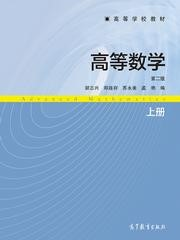
\includegraphics[width=\textwidth]{App1_1}
      \caption{上册.}
    \end{subfigure}
    \begin{subfigure}[b]{.23\textwidth}
      \centering
      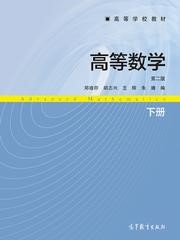
\includegraphics[width=\textwidth]{App1_2}
      \caption{下册.}
    \end{subfigure}
    \caption{北京科技大学 胡志兴等 编.高等数学(第二版),高等教育出版社.}\label{fig:教材}
  \end{figure}

  \hspace*{2em}再来说说如何入门。我们借一个例子来指出一些概念和知识上的错误,如\autoref{fig:一张错误的高等数学知识结构图}所示,
  \begin{figure}[!htb]
    \centering
    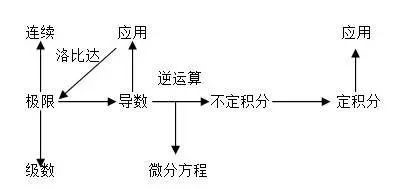
\includegraphics[width=.4\textwidth]{App1_3}
    \caption{一张错误的高等数学知识结构图.}\label{fig:一张错误的高等数学知识结构图}
  \end{figure}
  事实上,这张图不仅在内容上没有说清高等数学的梗概\footnote{应当包括一元函数微分学、一元函数积分学、向量代数与空间解析几何、多元函数微分学、多元函数积分学、无穷级数以及常微分方程七大板块,图中只提及了三个板块。}
  ,甚至在正确性上也令人怀疑。例如,极限是微积分的基础,用一个箭头从导数的应用指向极限,而这个箭头上标注着洛必达法则是合适的吗\footnote{作者的本意可能是指可以利用洛必达法则来计算函数的极限,但这仅仅是高等数学里一个非常细节性的知识点,把它放在概括高等数学全貌的知识结构图里是不合适的。}
  ?再如,导数与不定积分互为逆运算,为何没有用双向箭头连接?不是所有的定积分都可以通过不定积分计算(有的被积函数并不存在原函数,却是可积的),那么凭什么用一个箭头从不定积分指向定积分呢?这些问题尽管细节,却正说明这张图的作者并没有深入理解微积分这门学科里的概念,而只是浅尝辄止,至多停留于“考好即可”的地步。读者若想真正学好这门课,就绝不能有这样的想法——至少,课本上没有打星号指明可读可不读的章节,一定要反复读,学完之后还要回过头来思考各章节之间的联系。这样的学习甚至可能需要持续到本科高年级阶段。笔者在考研复习时整理的高等数学知识点结构图之某部分(未完成)如\autoref{fig:笔者在考研复习时整理的高等数学知识点结构图之某部分(未完成)}所示。
  \begin{figure}[!htb]
    \centering
    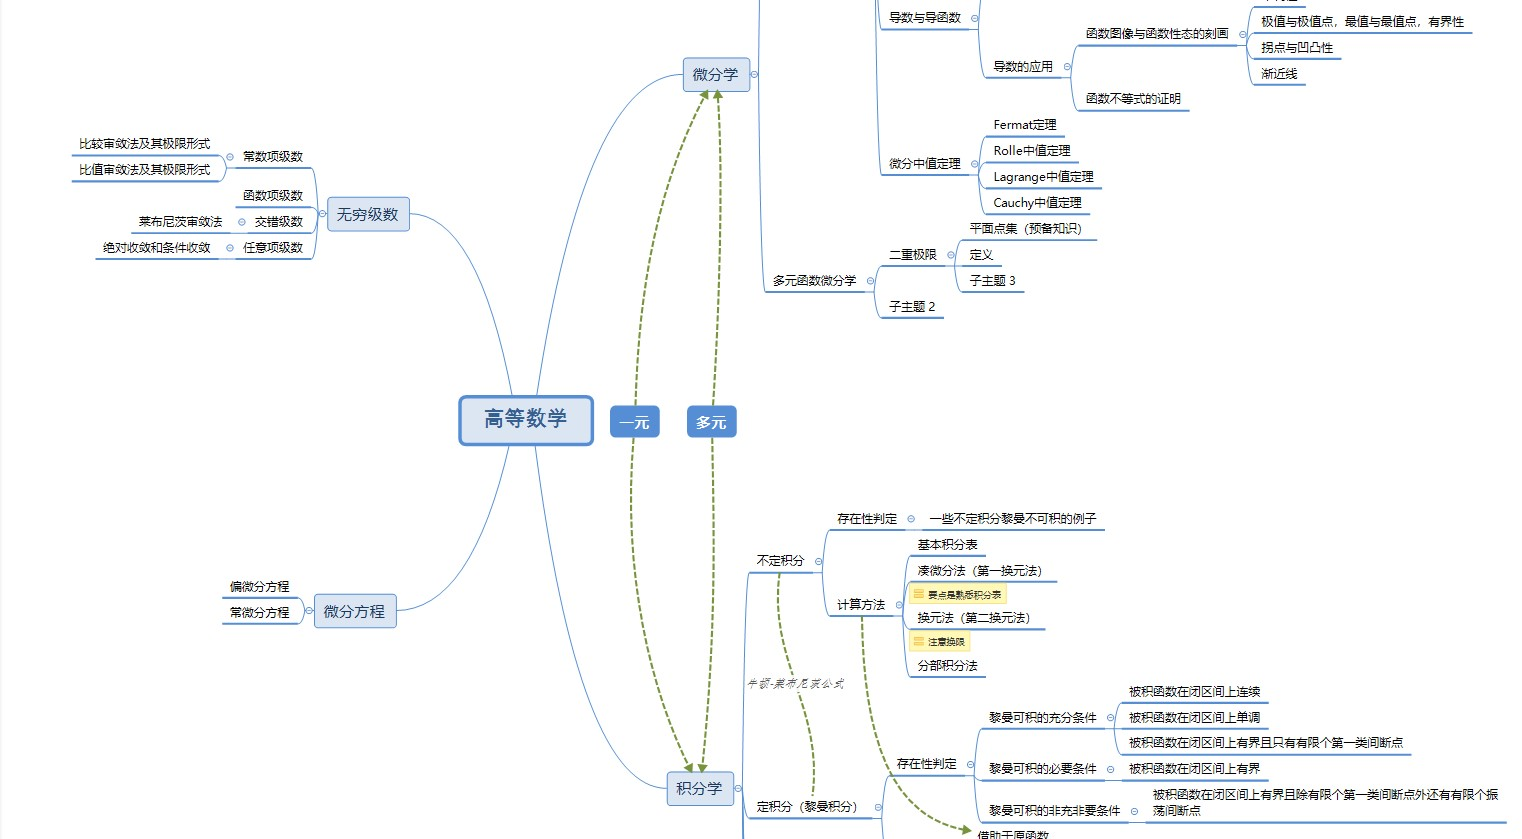
\includegraphics[width=.75\textwidth]{App1_4}
    \caption{笔者在考研复习时整理的高等数学知识点结构图之某部分(未完成).}\label{fig:笔者在考研复习时整理的高等数学知识点结构图之某部分(未完成)}
  \end{figure}

  \hspace*{2em}说完了这门学科大体上应当如何学习,我们再来聊点具体的、同时也是大家最关注的,那就是具体到课上课下时应该怎么做。笔者的经验是:高效的预习工作是每一轮学习中最重要的部分,课堂听讲抓住重点是必不可少的部分,课后及时的复习和总结是收获最大的部分。这样说是因为,高等数学这门课程抽象性比较强,概念多而且联系紧密、深刻而富有内涵,课程时间跨度大、强度大,课后练习题型丰富。尽管每年考试的题型大同小异,难度也很友好,但仍不能就此掉以轻心,而必须重视每一轮学习的每一个环节。

  \hspace*{2em}在课前预习部分,要做到了解下一堂课会提到哪些概念,这些概念同已经学过的部分有什么联系(例如,是从什么问题引出的,与之相关的命题是否能被前文所述的定理证明,等等);课堂上要重点关注两方面,一是老师是如何讲解自己在预习时尚未理解的部分,二是老师是如何解题的;课后复习要及时清完习题,以及再次阅读课本——对照老师在课堂上讲述的观点,以期加深理解、弥补不足。

  \hspace*{2em}在除教材以外的其他参考资料方面,学弟学妹们不必担心。自2009年自主编辑第一版《高等数学》、2013年修订编辑第二版《高等数学》,乃至学生讲师团建立以来,校内的各类资料可以说是无比丰富了。笔者自己使用过的纸质资料里,除物美复印店里可以找到的《高等数学练习册(2013版)》,以及期中、期末考试前讲师团发下的历年考试题外,还有其他一些学校的试卷,以及《吉米多维奇数学分析习题集学习指引》(谢惠民)、《高等数学复习指导——思路、方法与技巧》(陈文灯)、《大学生数学竞赛习题精讲》(陈兆斗)等等,至于电子版资料就更是数不胜数了,笔者使用过的部分电子版资料如\autoref{fig:笔者使用过的部分电子版资料}所示。
  \begin{figure}[!htb]
    \centering
    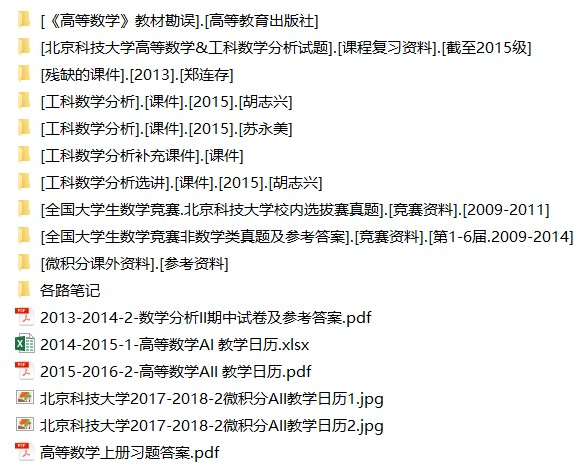
\includegraphics[width=.43\textwidth]{App1_5}
    \caption{笔者使用过的部分电子版资料.}\label{fig:笔者使用过的部分电子版资料}
  \end{figure}

  \hspace*{2em}总地来说,对于普通本科生而言,过于拔高习题的难度是没有太大意义的,但仅仅局限于课后习题也难以让学生深刻理解知识点(尽管我说的“深刻理解”可能不是读者以为的“深刻理解”)。斟酌再三,笔者认为在课后习题保质保量完成,而课余时间仍然充足的前提下,适当地看一些课外书、了解一些竞赛知识、做一些竞赛题是可以的,而刷大量的历年考试题则是没有必要的。个中滋味、如何平衡就待诸君正式开始学习之后,自行体会吧!

\section{学好高等数学有什么必要性以及帮助}
  \begin{marker}
  {\heiti 第三个问题:学习高等数学的意义在于什么?对于今后的学习、工作乃至生活有什么帮助?}
  \end{marker}

  \hspace*{2em}在谈论学习某一门学科的必要性之前,必须先了解这门学科的意义;而在了解其意义之后,“为什么要学习/不必学习这门课”也就不证自明了。

  \hspace*{2em}大而言之,冯·诺依曼在论述微积分时曾这样评价:“微积分是现代数学取得的最高成就,对它的重要性怎样估计也是不会过分的。”而今天,在微积分问世300余年之后,它依然值得被这样赞美——这不仅仅是因为其广泛而又重要的应用,更是由于人类在攀登这座高峰的历程中付出的艰辛努力,以及由此在思想史上写下的辉煌篇章。小而言之,今后几乎任何领域的研究工作的推进——从人工智能的训练模式到城市排水系统的改进,从航天器的设计到交通灯的安排……都要依靠、或者至少是借助数学工具,而微积分则是这些工具里最基础并且重要的之一。

  \hspace*{2em}以笔者自己学习专业课的经历为例,微积分工具乃至在大一大二其他课程里学习过的数学工具,在很多专业课里都有应用。例如,在经济学理论里经常要研究一些复杂的情况,这些情况通常被很多个因素影响。为了研究一种可变因素的数量变动会对其他可变因素的变动产生多大影响,需要用到边际分析方法,而“边际”这个概念回归到微积分理论里正是最基本的概念之一——导数。再如,理解计量经济学中的各种模型,需要先修微积分、线性代数、运筹学、概率论等多门基础数学课的知识,其中有一种GARCH模型,它应用于分析具有波动性集群效应的微观金融数据,或持有某项资产的风险(异方差)的情况。GARCH模型的基本形式GARCH$(p,q)$写为
  \begin{subnumcases}{}
    {y_t} = {{x'}_t}\phi  + {u_t}, \quad {u_t} \sim N\left( {0,\sigma _t^2} \right) \\
    \sigma _t^2 = {\alpha _0} + \sum_{i = 1}^p {{\alpha _i}u_{t - i}^2}  + \sum_{j = 1}^q {{\beta _j}\sigma _{t - j}^2} \label{equ:GARCH}
  \end{subnumcases}
  在平稳随机过程的条件下\autoref{equ:GARCH}也可以写成
  $\sigma _t^2 = \beta {\left( L \right)^{ - 1}}{\alpha _0} + \beta {\left( L \right)^{ - 1}}\alpha \left( L \right)u_t^2$
  的形式,而这两种形式之间的变换则要涉及到微分算子\footnote{读者将会在大一年级下学期的《高等数学\ROMAN{1}》或《工科数学分析\ROMAN{2}》课程里首次接触到“微分算子”的概念。}
  的概念了。定义这样一个平稳过程中的滞后算子:
  \[ \begin{cases}
    \alpha \left( L \right) = {\alpha _1}L + {\alpha _2}{L^2} +  \cdots  + {\alpha _p}{L^p} \hfill \\
    \beta \left( L \right) = 1 - {\beta _1}L - {\beta _2}{L^2} -  \cdots  - {\beta _p}{L^p}
  \end{cases} \]
  \hspace*{2em}于是有
  $\beta \left( L \right)\sigma _t^2 = {\alpha _0} + \alpha \left( L \right)u_t^2$
  ,代入\autoref{equ:GARCH}便得到其变换后的形式。

  再如,对于借助计算机研究各种工程现象的工程人员来讲,求解一个代数方程通常要比求解一个微分方程容易得多,而要将微分方程转化为代数方程则需要使用积分变换的方法。例如,经典控制理论中对控制系统的分析和综合都建立在Laplace变换的基础上,而引入拉普拉斯变换的一个主要优点,是可以用传递函数代替常系数微分方程来描述系统的特性,为采用直观和简便的图解方法来确定控制系统特性、分析控制系统的运动过程,以及控制系统的参数整定提供极大的便利。而要想理解Laplace变换,就必须先修微积分课程里的积分学,并深入理解复变函数的概念和性质。

  \hspace*{2em}当然,也有同学志不在科研或深造,而是希望毕业之后投身职业圈——怀有这样志向的学生并不少见,也并无可指摘之处,但若就此认为大学里的高等数学(乃至某些其他必修课程)是没有必要学习的,那笔者只好送他们一句流传甚广的玩笑话了:“数学不能用来买菜,却可以决定你在哪里买菜。”

\section{一些笔者推荐的课外数学资料}
~
  \subsection{书籍}
    \hspace*{2em}必须事先指出的是,以下这些书籍不一定对“使课程取得高分”有用,而仅以飨读者之思想。排名不分先后,尽可凭兴趣阅读。
  \begin{enumerate}[label=(\arabic*),leftmargin=4em]
    \item 《数学——它的内容、方法和意义》[俄]A.D.亚历山大洛夫 等 著

    本书由前苏联数位著名数学家为普及数学知识而合力撰写,介绍了现代数学各个分支的内容、历史发展及其在自然科学和工程技术中的应用,语言通俗简练,内容由浅入深,可供高等院校理工科师生、普通高中师生、工程技术人员和数学爱好者阅读。

    \item 《古今数学思想》[美]Morris Klein 著

    本书论述了从古代一直到20世纪头几十年中的重大数学创造和发展,目的是介绍中心思想,特别着重于那些在数学历史的主要时期中逐渐冒出来并成为最突出的、并且对于促进和形成尔后的数学活动有影响的主流工作。不同于一般数学史的著作,而主要作为“从历史角度来讲解的数学入门书”,该书突出了数学发展历程中涌现的各类思想方法,论述了数学思想的古往今来,被誉为“我们现有的数学史中最好的一本数学史”。

    \item 《微积分的历程:从牛顿到勒贝格》[美]William Dunham 著

    本书宛如一座陈列室,汇聚了十多位数学大师的杰作,当你徜徉其中时会对人类的想象力惊叹不已,当你离去时必然满怀对天才们的钦佩感激之情。作者同读者一起分享了分析学历史中为人景仰的理论成果。书中的每一个结果,从牛顿的正弦函数的推导,到伽玛函数的表示,再到贝尔的分类定理,无一不处于各个时代的研究前沿,至今还闪烁着耀眼夺目的光芒。
  \end{enumerate}
    \begin{figure}[!htb]
      % \centering
    \hfill
    \begin{subfigure}[b]{.23\textwidth}
      \centering
      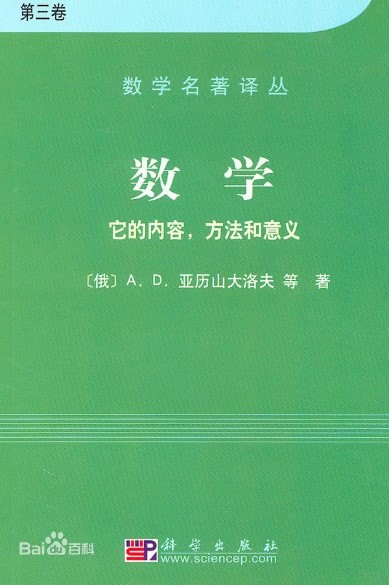
\includegraphics[width=\textwidth]{App1_6}
      \caption{《数学——它的内容、方法和意义》[俄]A.D.亚历山大洛夫 等 著.}
    \end{subfigure}
    \hfill
    \begin{subfigure}[b]{.23\textwidth}
      \centering
      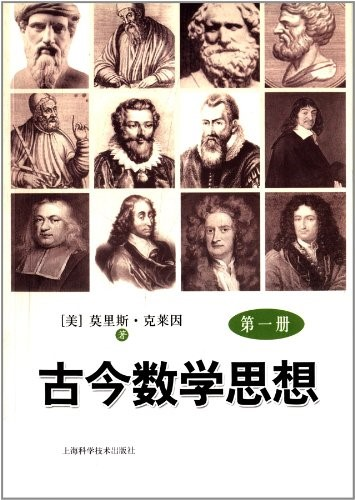
\includegraphics[width=\textwidth]{App1_7}
      \caption{《古今数学思想》[美]Morris Klein 著.}
    \end{subfigure}
    \hfill
    \begin{subfigure}[b]{.23\textwidth}
      \centering
      
\includegraphics[width=\textwidth]{App1_8}
      \caption{《微积分的历程:从牛顿到勒贝格》[美]William Dunham 著.}
    \end{subfigure}
    \caption{笔者推荐的部分书目.}
  \end{figure}
  \hspace*{2em}当然,好书还有很多,为免贪多嚼不烂,笔者就不一一列举了。

  \subsection{公共资源平台}
    \hspace*{2em}除去本校学生讲师团为每届学弟学妹们建立的数学交流群之外,还有许多公共平台可以为希望提高自身数学水平(以在期末考试乃至数学竞赛中取得好成绩)的大学生提供各类学习资源,包括书籍、习题、文章等等。例如\autoref{fig:笔者推荐的部分微信公众号}所示微信公众号。
    \begin{figure}[!htb]
    \centering
    \hfill
    \begin{subfigure}[b]{.23\textwidth}
      \centering
      
\includegraphics[width=\textwidth]{App1_9}
      \caption{高等数学.}
    \end{subfigure}
    \hfill
    \begin{subfigure}[b]{.23\textwidth}
      \centering
      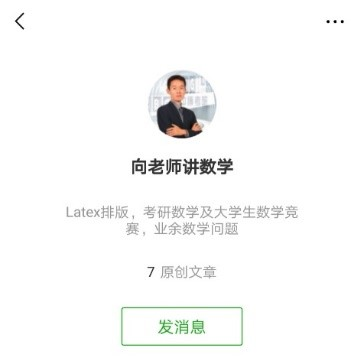
\includegraphics[width=\textwidth]{App1_10}
      \caption{向老师讲数学.}
    \end{subfigure}
    \hfill
    \begin{subfigure}[b]{.23\textwidth}
      \centering
      
\includegraphics[width=\textwidth]{App1_11}
      \caption{考研竞赛数学.}
    \end{subfigure}
    \hfill
    \begin{subfigure}[b]{.23\textwidth}
      \centering
      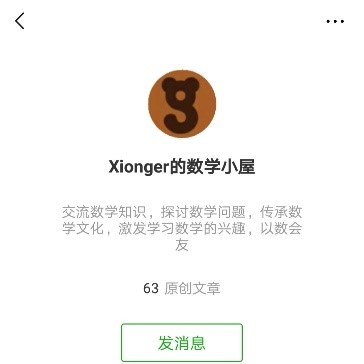
\includegraphics[width=\textwidth]{App1_12}
      \caption{Xionger的数学小屋.}
    \end{subfigure}
    \caption{笔者推荐的部分微信公众号.}\label{fig:笔者推荐的部分微信公众号}
    \end{figure}

    \hspace*{2em}有兴趣的学弟学妹们也可以自行搜索各种数学交流群(我的经验告诉我,大佬们都在各个QQ群里交流,就看你有没有本事加进去了),这里就不赘述了。
